\documentclass[12pt]{article}
\usepackage[margin=0.3in,top=0.25in,bottom=0.4in]{geometry}
\makeatletter
\renewcommand{\@maketitle}{\newpage\null\vskip -3.5em\begin{center}{\LARGE \@title \par}\end{center}\par\vskip 0.2em}
\makeatother
\usepackage{amsmath,amssymb}
\usepackage{booktabs}
\usepackage{hyperref}
\usepackage{graphicx}
\setlength{\parskip}{0.6em}
\setlength{\parindent}{0pt}
\newcommand{\xpo}{x_{\mathbb{P}}}

\title{The diffractive (TMD) cross section after the fix:\\
flat in $\ln\xpo$, larger than the exclusive one, and rapidity dependent}
\author{}
\date{}

\begin{document}
\maketitle

\section*{In short}

After the fix of the diffractive integrand (gluon dipole $\mathcal{N}_g$ and the measure
$\mathrm{d}\ln\xpo$), three features of our results are worth understanding:
\begin{enumerate}
\item $\mathrm{d}\sigma/\mathrm{d}\ln\xpo$ is nearly \textbf{flat} above a kinematic edge, and at fixed
  $z$ the curves for different rapidities \textbf{approach the same plateau} at large $\xpo$ (they do
  not coincide elsewhere);
\item the diffractive (TMD) cross section is \textbf{larger than the exclusive one} from
  $p_\perp\approx1$~GeV on;
\item it depends \textbf{more strongly on rapidity} than before.
\end{enumerate}
All three follow from the formula of Ref.~[3] and the kinematics. Section~0 collects what is needed
to follow the rest; the references are listed at the end.

\section*{0. Setup: the two processes and the formulas}

\textbf{The processes.} A quasi-real photon ($Q^2\simeq0$) from one nucleus hits the other nucleus
(or a proton), which stays intact (coherent diffraction). A rapidity gap
$Y_{\mathbb{P}}=\ln(1/\xpo)$ separates the target from the produced system: the colourless exchange
(the ``Pomeron'') carries a fraction $\xpo$ of the target nucleon momentum.
\begin{itemize}
\item \textbf{Exclusive}, $\gamma+A\to c\bar c+A$: only the charm pair is produced.
\item \textbf{Diffractive (TMD)}, $\gamma+A\to c\bar c g+A$: a hard $c\bar c$ pair plus a soft gluon.
  For $p_\perp\gg Q_s$ it factorizes into a hard factor times the gluon distribution of the Pomeron
  (a ``diffractive TMD'', DTMD) [3].
\end{itemize}

\textbf{Kinematics} (light-cone variables, as in the draft). The photon moves in the $+z$ direction
with momentum $q^+$; positive rapidity $y$ is the photon direction.
\begin{center}
\begin{tabular}{ll}
\toprule
$\mathbf{p}$, $p_\perp$ & transverse momentum of the charm quark \\
$z=p^+/q^+$ & quark momentum fraction w.r.t.\ the photon; $p^+=m_te^y/\sqrt2$, $m_t=\sqrt{p_\perp^2+m^2}$ \\
$W^2=2q^+P_N^-$ & photon--nucleon energy squared \\
$M_{q\bar q}^2=m_t^2/[z(1-z)]$ & invariant mass of the pair \\
$x_{q\bar q}=M_{q\bar q}^2/W^2$ & the smallest possible $\xpo$ (exclusive: $\xpo=x_{q\bar q}$) \\
$x=x_{q\bar q}/\xpo$ & fraction of the Pomeron momentum carried by the $t$-channel gluon \\
$\mathbf{K}$, $K_\perp$ & momentum imbalance of the pair $=$ minus the soft-gluon momentum \\
$z_\gamma=\omega/E_A$ & photon energy fraction; flux $F(z_\gamma)=\mathrm{d}N/\mathrm{d}z_\gamma$ \\
\bottomrule
\end{tabular}
\end{center}

\textbf{The target.} $\mathcal{N}(R,\xpo)$ is the scattering amplitude of a quark--antiquark dipole of
size $R$ (BK-evolved, MVe initial condition), and $\mathcal{N}_g=2\mathcal{N}-\mathcal{N}^2$ that of a
gluon--gluon dipole. For small dipoles $\mathcal{N}\simeq Q_s^2R^2/4$ (up to a logarithm); for
$R\gtrsim1/Q_s$, $\mathcal{N}\to1$ (saturation). $Q_s$ is the saturation scale, $Q_s^2\sim0.5$--1
GeV$^2$ here. In our code $\xpo\leq0.1$, and the dipole is frozen at $\xpo=0.01$ for
$0.01<\xpo\leq0.1$.

\textbf{Exclusive cross section} (Eq.~(1) of the draft; Ref.~[2] for $m=0$):
\[
  \frac{\mathrm{d}\sigma^{\rm excl}}{\mathrm{d}y\,\mathrm{d}^2\mathbf{p}}
  =\frac{\alpha_{\rm em}e_c^2N_cS_\perp m^2}{2\pi^2}\,z\Big[(z^2+\bar z^2)\,I_1^2+I_0^2\Big],\qquad
  I_\nu=\int_0^\infty\mathrm{d}R\,R\,J_\nu(p_\perp R)\,K_\nu(mR)\,\mathcal{N}(R,\xpo)\,,
\]
with $\bar z=1-z$ and $\xpo=x_{q\bar q}$ fixed by the kinematics.

\textbf{Diffractive (TMD) cross section} (Eqs.~(3.38), (3.39), (3.43)--(3.45) of Ref.~[3], $Q^2=0$):
\[
  \frac{\mathrm{d}\sigma^{\rm diff}}{\mathrm{d}z_1\mathrm{d}z_2\,\mathrm{d}^2\mathbf{K}\,\mathrm{d}^2\mathbf{P}\,\mathrm{d}\ln(1/x)}
  =\mathcal{H}(z,P_\perp)\,\frac{\mathrm{d}\,xG_{\mathbb{P}}(x,\xpo,K_\perp)}{\mathrm{d}^2K}\,,
\]
\[
  \mathcal{H}=\alpha_{\rm em}\alpha_s\,e_c^2\left[(z^2+\bar z^2)\frac{P_\perp^4+m^4}{(P_\perp^2+m^2)^4}
  +\frac{2m^2P_\perp^2}{(P_\perp^2+m^2)^4}\right]\;\xrightarrow{P_\perp\gg m}\;\frac{\alpha_{\rm em}\alpha_se_c^2(z^2+\bar z^2)}{P_\perp^4}\,,
\]
\[
  \frac{\mathrm{d}\,xG_{\mathbb{P}}}{\mathrm{d}^2K}=\frac{S_\perp(N_c^2-1)}{8\pi^4}\,\frac{G^2}{1-x}\,,\qquad
  G=\Omega^2\int_0^\infty\mathrm{d}R\,R\,J_2(K_\perp R)\,K_2(\Omega R)\,\mathcal{N}_g(R,\xpo)\,,\qquad
  \Omega^2=\frac{x}{1-x}K_\perp^2\,.
\]
For a given photon energy and fixed quark kinematics, $\mathrm{d}\ln(1/x)=\mathrm{d}\ln\xpo$, so the
right-hand side is $\mathrm{d}\sigma/\mathrm{d}\ln\xpo$, and the cross section is
$\int\mathrm{d}\ln\xpo$ from $\xpo^{\min}\simeq x_{q\bar q}$ to $\xpo^{\max}=0.1$, and
$\int\mathrm{d}^2K$ up to $K_\perp\leq p_\perp$. In a UPC the result is then integrated over the photon
energy with $F(z_\gamma)$.

\section*{1. Why $\mathrm{d}\sigma/\mathrm{d}\ln\xpo$ is flat}

\begin{figure}[h]
\centering
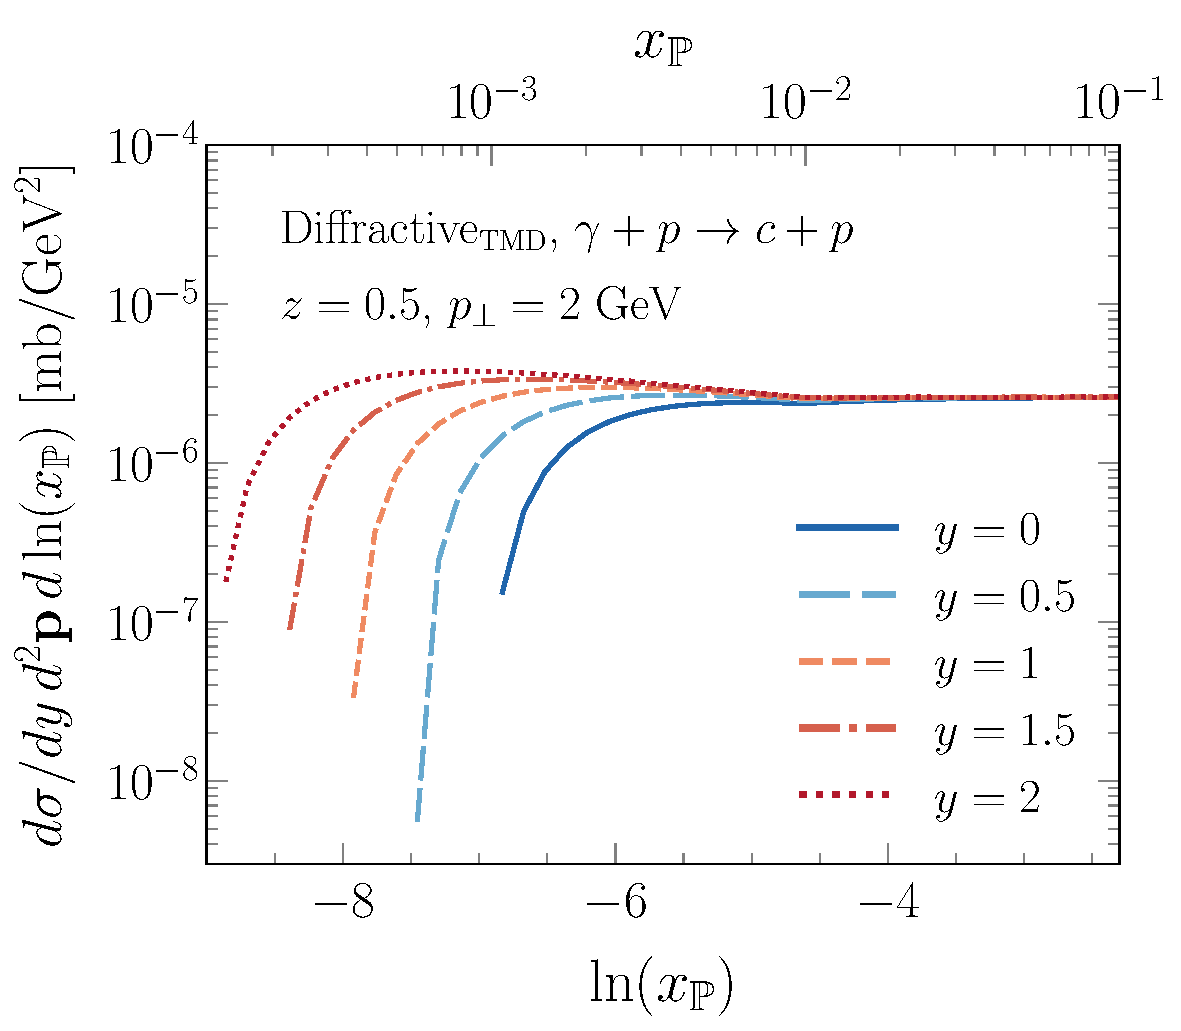
\includegraphics[width=0.48\textwidth]{../plots/charm_fixed_qp_xpom.pdf}\hfill
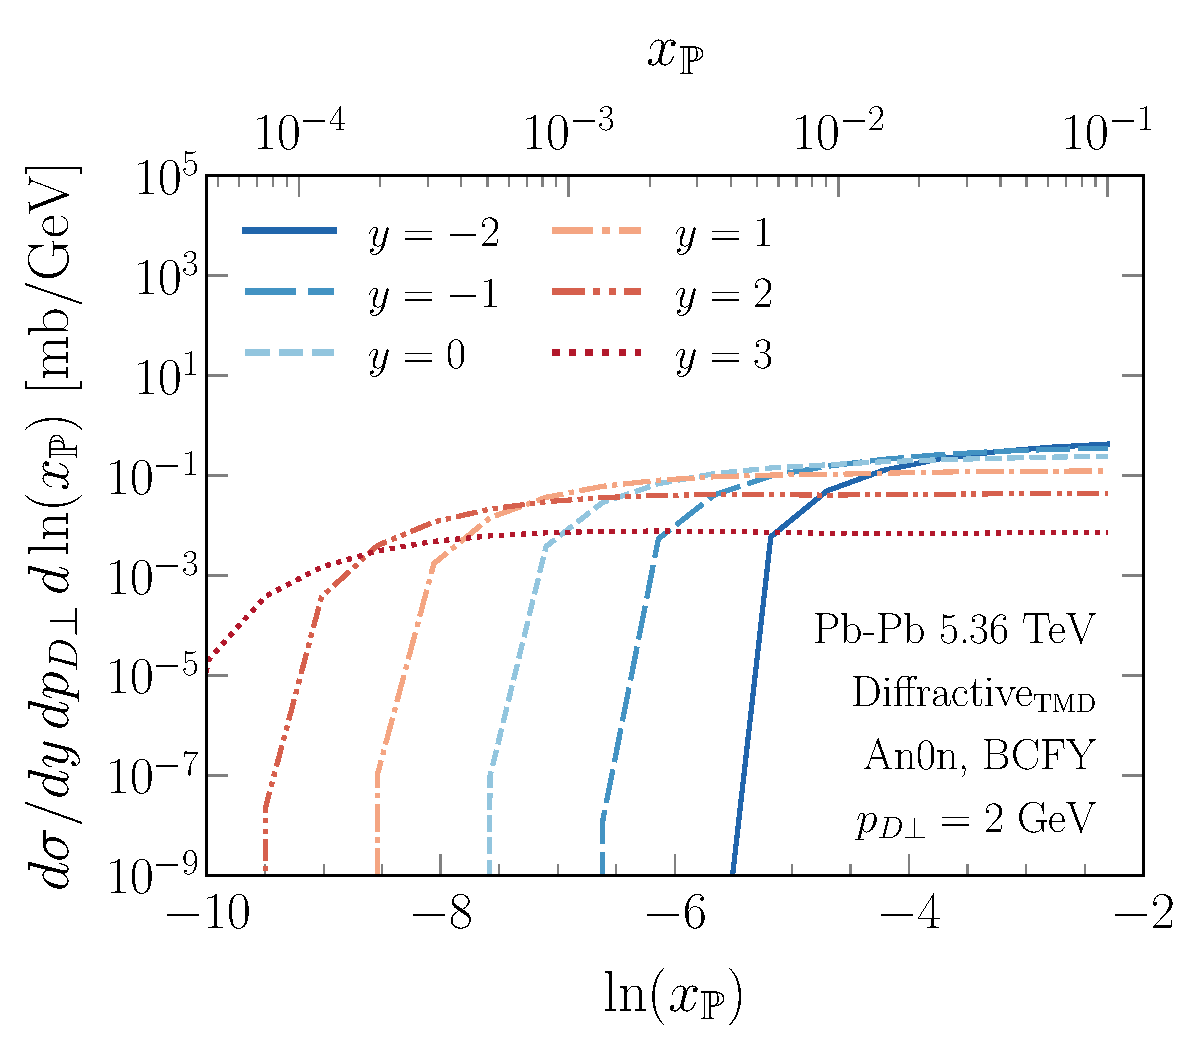
\includegraphics[width=0.48\textwidth]{../plots/xpom_An0n_PbPb.pdf}
\caption{$\mathrm{d}\sigma/\mathrm{d}\ln\xpo$ against $\ln\xpo$. Left: charm quark, $\gamma+p$ at fixed
$z=0.5$ ($q^+=2p^+$, one photon energy per rapidity) and $p_\perp=2$~GeV. Right: $D^0$ in Pb--Pb UPCs (An0n, BCFY,
$p_{D\perp}=2$~GeV). The area under each curve is the cross section.}
\end{figure}

\textbf{Large $\xpo$ means small $x$.} For a given photon and given quark kinematics,
$x_{q\bar q}\equiv M_{q\bar q}^2/W^2$ is fixed, and
\[
  x=\frac{x_{q\bar q}}{\xpo}\,.
\]
Moving to the right in the $\xpo$ figure therefore sends $x\to0$.

\textbf{At small $x$ the Pomeron gluon distribution does not depend on $x$.} The $x$ dependence of
\[
  G=\Omega^2\int_0^\infty\mathrm{d}R\,R\,J_2(K_\perp R)\,K_2(\Omega R)\,\mathcal{N}_g(R,\xpo)
\]
is only through $\Omega$. For $x\to0$, $\Omega\to0$ and $K_2(\Omega R)\approx2/(\Omega R)^2$, so the
$\Omega^2$ in front cancels:
\[
  G\;\longrightarrow\;2\int_0^\infty\frac{\mathrm{d}R}{R}\,J_2(K_\perp R)\,\mathcal{N}_g(R,\xpo)\,,
\]
independent of $x$; also $1/(1-x)\to1$. The diffractive gluon distribution $\mathrm{d}\,xG_{\mathbb{P}}/\mathrm{d}^2K$
of Eq.~(3.45) of Ref.~[3] reaches a plateau. (Ref.~[3] stresses that $x$ enters only through
$\Omega$, Eq.~(3.39); the limit above follows from $K_2(u)\simeq2/u^2$ for $u\to0$.)

\textbf{The remaining $\xpo$ dependence is weak.} It is only in $\mathcal{N}_g(R,\xpo)$: slow BK
evolution for $\xpo<0.01$, and none for $0.01<\xpo\leq0.1$, where the dipole is frozen at
$\xpo=0.01$. So, once $x\ll1$, the curve is nearly flat below $\xpo=0.01$ (it decreases slowly with
$\xpo$, because the dipole is larger at smaller $\xpo$: for $y=2$ it is 24\% higher at $\xpo=10^{-3}$
than at $10^{-2}$) and exactly flat above.

\textbf{The steep edge on the left} is the opposite limit: when $\xpo\to x_{q\bar q}$, $x\to1$,
$\Omega\to\infty$ and $K_2(\Omega R)$ suppresses $G$ exponentially. Below
$\xpo=x_{q\bar q}$ the process is not possible.

\textbf{How the rapidities compare.} A remark on the name first: the charm figures are at fixed
$z=0.5$ ($q^+=2p^+$) and $p_\perp=2$~GeV. Each curve has one photon energy, but it is different for
each rapidity ($q^+=\sqrt2\,m_te^y$); ``fixed photon energy'' means that it is not integrated over.

The curves for different rapidities do \emph{not} coincide in general. The hard factor
$\mathcal{H}(z,p_\perp)$ is the same for all of them, but $x=x_{q\bar q}/\xpo$ is not: at a given
$\xpo$, a smaller rapidity has a larger $x_{q\bar q}$ and hence a larger $x$, and the gluon
distribution is smaller (roughly like $1-x$, Sec.~1b). They only approach a common value where
$x\ll1$ for all of them, i.e.\ towards $\xpo=0.1$:
\begin{center}
\begin{tabular}{cccc}
\toprule
$\xpo$ & $x$ for $y=0$ / $y=2$ & ($y=0$)/($y=2$) & ($y=1$)/($y=2$) \\
\midrule
$10^{-3}$ & 0.93 / 0.13 & 0.02 & 0.67 \\
$3\times10^{-3}$ & 0.31 / 0.04 & 0.64 & 0.91 \\
$10^{-2}$ & 0.09 / 0.013 & 0.91 & 0.98 \\
$3\times10^{-2}$ & 0.03 / 0.004 & 0.97 & 0.99 \\
$10^{-1}$ & 0.009 / 0.001 & 0.99 & 1.00 \\
\bottomrule
\end{tabular}
\end{center}
(ratios of $\mathrm{d}\sigma/\mathrm{d}\ln\xpo$ from our runs). At $\xpo=0.01$ the $y=0$ curve is still
9\% below the $y=2$ one, as expected from $1-x=0.91$. So the curves merge only at the right end of
the figure; over most of the range they differ, and most of all near the edge.

\textbf{Consequence.} Well above the edge, every unit of $\ln\xpo$ contributes about the same, so
\[
  \sigma\;\approx\;(\text{plateau height})\times\ln\frac{\xpo^{\max}}{\xpo^{\min}}
  \;+\;(\text{edge})\,,\qquad \xpo^{\min}\simeq x_{q\bar q}\,.
\]
This is why the upper cut ($\xpo^{\max}=0.1$ or $0.04$) matters, as also found by Guzey et al.\
(arXiv:2606.05469).

\subsection*{1b. The same result in momentum space, and in the literature}

\textbf{Saturated region, exactly.} Where $\mathcal{N}_g=1$, the $R$ integral can be done for any $x$,
using $\int_0^\infty\mathrm{d}R\,R\,J_\nu(aR)K_\nu(bR)=(a/b)^\nu/(a^2+b^2)$ with $\Omega^2/K_\perp^2=x/(1-x)$:
\[
  G=\Omega^2\int_0^\infty\mathrm{d}R\,R\,J_2(K_\perp R)\,K_2(\Omega R)=1-x\,,
  \qquad
  \frac{\mathrm{d}\,xG_{\mathbb{P}}}{\mathrm{d}^2K}\propto\frac{G^2}{1-x}=1-x\,.
\]
This is the first line of Eq.~(19) in Iancu et al.\ (arXiv:2304.12401). It goes to a constant for
$x\to0$ and vanishes for $x\to1$.

\textbf{Momentum space (Appendix D of Ref.~[3]).} Eq.~(D.7) at $\Delta=0$ reads, schematically,
\[
  \frac{\mathrm{d}\,xG_{\mathbb{P}}}{\mathrm{d}^2K}\propto(N_c^2-1)(1-x)\int\mathrm{d}^2q\,\mathrm{d}^2q'\,
  D_A(q)D_A^*(q')
  \left[\frac{2K^nK^m-K^2\delta^{nm}}{K^2}
  -\frac{2(K+q)^n(K+q)^m-(K+q)^2\delta^{nm}}{(1-x)(K+q)^2+xK^2}\right]\times\big[\,q\to q'\,\big]\,.
\]
Here $x$ appears explicitly. For $x\to0$ the denominators become $K^2$ and $(K+q)^2$, independent of
$x$: the gluon DTMD tends to a constant. For $x\to1$ the prefactor $(1-x)$ makes it vanish (the edge).
Ref.~[3] gives this expression but does not discuss the limit.

\textbf{Quark vs.\ gluon.} Appendix~C.2 of Ref.~[3] gives the exact $x\to0$ limit of the
\emph{quark} DTMD (Eq.~(C.29), $m=0$): it is proportional to $x$ and vanishes. The \emph{gluon} DTMD
instead tends to a constant. Since our cross section is
$\mathrm{d}\sigma/\mathrm{d}\ln\xpo=\mathcal{H}\,\mathrm{d}\,xG_{\mathbb{P}}/\mathrm{d}^2K$, it is the constant
gluon DTMD at small $x$ that makes $\mathrm{d}\sigma/\mathrm{d}\ln\xpo$ flat at large $\xpo$.

\textbf{Iancu, Mueller, Triantafyllopoulos and Wei.} The small-$x$ behaviour of the gluon DTMD is
discussed explicitly in their papers:
\begin{itemize}
\item \emph{Gluon dipole factorisation for diffractive dijets}, JHEP 10 (2022) 103
  (arXiv:2207.06268; Ref.~[14] of Ref.~[3]), Sec.~5. The $K_\perp$-integrated distribution is
  \[
    xG_{\mathbb{P}}(x,\xpo,P_\perp^2\to\infty)=\frac{S_\perp(N_c^2-1)}{4\pi^3}\,\kappa(x)\,(1-x)\,\tilde Q_s^2(x,Y_{\mathbb{P}})\,,
    \qquad\tilde Q_s^2(x)=(1-x)\,Q_s^2\,,
  \]
  Eq.~(5.19), with $\kappa(x)$ slowly varying: in the GBW model $\kappa(0)\simeq0.693$ and
  $\kappa(1)\simeq1.345$. So the tree-level distribution tends to the constant $\kappa(0)Q_s^2(Y_{\mathbb{P}})$
  (times $S_\perp(N_c^2-1)/4\pi^3$) for $x\to0$, and vanishes like $(1-x)^2$ for $x\to1$ (``the
  Pomeron as being built with 2 constituent gluons''). In the dilute tail, Eq.~(5.8),
  $G\simeq(1-x)(1+2x)\,\tilde Q_s^2(x)/K_\perp^2$, again finite at $x\to0$.
\item \emph{Probing parton saturation and the gluon dipole via diffractive jet production at the
  EIC}, PRL 128 (2022) 202001 (arXiv:2112.06353), Eq.~(20): $xG_{\mathbb{P}}=S_\perp(1-x)^2\,
  \frac{N_c^2-1}{(2\pi)^3}\,\kappa\,Q_s^2(Y_{\mathbb{P}})$.
\item \emph{Probing gluon saturation via diffractive jets in ultra-peripheral nucleus-nucleus
  collisions} (arXiv:2304.12401): the cross section is written per $\mathrm{d}\ln(1/x)$ using
  $\mathrm{d}Y_{\mathbb{P}}=\mathrm{d}\ln(1/x)$ (their Eq.~(34)), the same measure as ours; in the MV
  model ``the gluon distribution of the Pomeron is independent of $\xpo$''.
\end{itemize}

\textbf{Beyond tree level.} Iancu et al.\ also show that DGLAP evolution of the Pomeron gluon
distribution from $Q_s^2$ to $P_\perp^2$ makes it \emph{grow} at small $x$, in a double-logarithmic way,
Eq.~(5.28) of arXiv:2207.06268, and suppresses it faster near $x=1$. Our calculation uses the
tree-level gluon DTMD of Ref.~[3], without this evolution, so it has the flat plateau. With DGLAP
evolution, the small-$x$ (large-$\xpo$) region would be enhanced further, and the dependence on
$\xpo^{\max}$ would become even stronger.

\section*{2. Why the diffractive (TMD) cross section is larger than the exclusive one}

The two processes fall differently with $p_\perp$: for charm photoproduction the exclusive one like
$p_\perp^{-8}$ (higher twist, with an extra mass suppression), the diffractive TMD one like
$p_\perp^{-4}$ (leading twist). Ref.~[2] (Sec.~1) states that the exclusive contribution
``decreases like the power $1/P_\perp^6$'', ``related to the colour transparency of small colour
dipoles''; that power holds when the photon wavefunction has a scale of order $P_\perp$ (DIS with
$Q^2\sim P_\perp^2$). In photoproduction the only scale of the photon wavefunction is the quark mass,
which gives two more powers of $m/p_\perp$ (below).

\textbf{Exclusive, $\gamma\to c\bar c$: the target must supply all the momentum.} The $c$ and
$\bar c$ come out back-to-back with $\pm\mathbf{p}$, so the target has to give transverse momentum
$\sim p_\perp$ to a colour-neutral pair. This needs a small dipole, $R\sim1/p_\perp$, for which the
amplitude is dilute, $\mathcal{N}\simeq Q_s^2R^2/4$ (up to a logarithm). Our cross section,
Eq.~(1) of the draft, is
\[
  \frac{\mathrm{d}\sigma}{\mathrm{d}y\,\mathrm{d}^2\mathbf{p}}\propto m^2\Big[(z^2+\bar z^2)\,I_1^2+I_0^2\Big],\qquad
  I_\nu=\int_0^\infty\mathrm{d}R\,R\,J_\nu(p_\perp R)\,K_\nu(mR)\,\mathcal{N}(R)\,,
\]
which is the massive photon wavefunction $(z^2+\bar z^2)\,\epsilon^2K_1^2(\epsilon r)+m^2K_0^2(\epsilon r)$ at
$Q^2=0$ ($\epsilon=m$), and reduces to Eq.~(2.23) of Ref.~[2] (with $\bar Q\to m$) for the first term.
With $\mathcal{N}=Q_s^2R^2/4$ the integrals are known in closed form,
\[
  I_1=\frac{2\,Q_s^2\,p_\perp m}{(p_\perp^2+m^2)^3}\simeq\frac{2Q_s^2m}{p_\perp^5}\,,\qquad
  I_0=\frac{Q_s^2\,(m^2-p_\perp^2)}{(p_\perp^2+m^2)^3}\simeq-\frac{Q_s^2}{p_\perp^4}\,,
\]
so at large $p_\perp$ the helicity-flip (mass) term $m^2I_0^2$ dominates:
\[
  \frac{\mathrm{d}\sigma^{\rm excl}}{\mathrm{d}y\,\mathrm{d}^2\mathbf{p}}\;\propto\;\frac{m^2\,Q_s^4}{p_\perp^8}
  \qquad\Big(\text{the }(z^2+\bar z^2)\text{ term is }\propto m^4Q_s^4/p_\perp^{10}\Big).
\]
For comparison, in DIS with a massless quark the first term is $\bar Q^2I_1^2\propto\bar Q^4Q_s^4/p_\perp^{10}$,
which becomes the $Q_s^4/p_\perp^6$ of Ref.~[2] when $\bar Q\sim p_\perp$.

\begin{figure}[h]
\centering
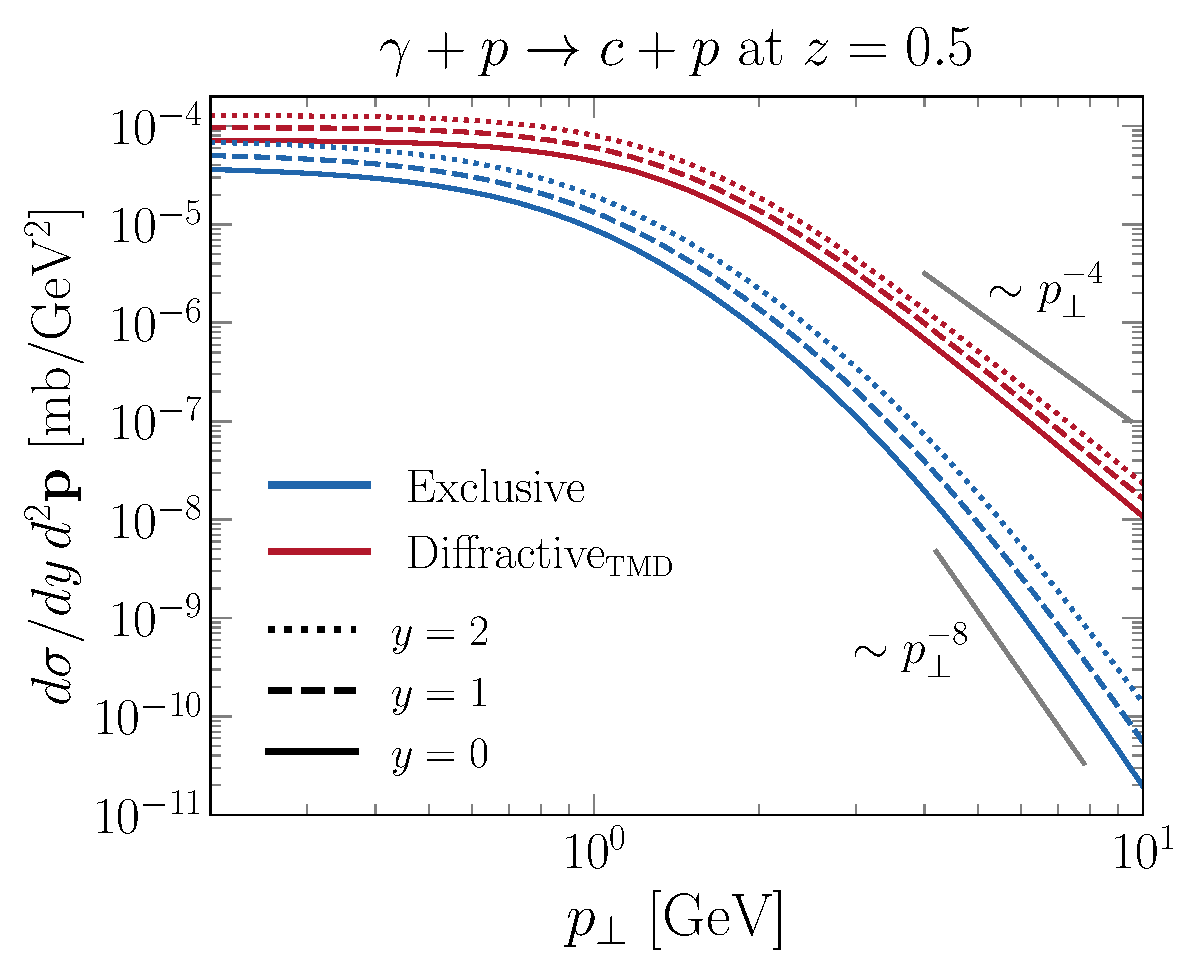
\includegraphics[width=0.55\textwidth]{../plots/charm_fixed_qp.pdf}
\caption{Charm quark, $\gamma+p$ at fixed $z=0.5$ ($q^+=2p^+$): exclusive (blue) and diffractive
TMD (red), with the guide lines $p_\perp^{-8}$ and $p_\perp^{-4}$.}
\end{figure}

\textbf{Check with our results} (charm at fixed $q^+$, $z=0.5$, $y=0$; local slope
$\mathrm{d}\ln\sigma/\mathrm{d}\ln p_\perp$ of $\mathrm{d}\sigma/\mathrm{d}y\,\mathrm{d}^2\mathbf{p}$):
\begin{center}
\begin{tabular}{cccccc}
\toprule
$p_\perp$ [GeV] & 2--4 & 4--6 & 6--10 & 10--15 & 15--20 \\
\midrule
exclusive   & $-5.4$ & $-7.0$ & $-8.0$ & $-8.2$ & $-9.0$ \\
diffractive & $-3.7$ & $-4.4$ & $-4.6$ & $-4.6$ & $-4.9$ \\
\bottomrule
\end{tabular}
\end{center}
The exclusive part reaches $p_\perp^{-8}$ only above $\sim6$~GeV (below, $p_\perp$ is not much larger
than $m$ and $Q_s$). The diffractive one is a little steeper than $p_\perp^{-4}$ because of the running
of $\alpha_s(m_t)$ and because the $\ln\xpo$ range shrinks as $x_{q\bar q}\propto m_t^2$ grows. (For
$\mathrm{d}\sigma/\mathrm{d}y\,\mathrm{d}p_\perp$, as in the $D^0$ plots, all powers are one unit
smaller: $p_\perp^{-7}$ and $p_\perp^{-3}$.)

\textbf{Diffractive, $\gamma\to c\bar cg$: the gluon takes the recoil.} The hard $c\bar c$ pair is
made by the photon splitting, in $\mathcal{H}(z,p_\perp)\propto1/p_\perp^4$. The target only provides
a soft gluon with $K_\perp\sim Q_s$, which balances the momentum. The target never has to supply the
large $p_\perp$, so there is no $Q_s^2/p_\perp^2$ penalty. In Ref.~[3]: the gluon is emitted at a
distance $R\sim1/K_\perp\sim1/Q_s$, large enough ``to allow for strong scattering and thus avoid the
suppression due to colour transparency''. The hard factor, Eq.~(3.44) of Ref.~[3], contains
$\alpha_s$ and behaves as $1/P_\perp^4$ for $P_\perp\gg m$.

\textbf{Size of the ratio.} Roughly,
\[
  \frac{\sigma_{\rm diff}}{\sigma_{\rm excl}}\;\sim\;\alpha_s\times\frac{p_\perp^4}{m^2Q_s^2}
  \times\ln\frac{\xpo^{\max}}{\xpo^{\min}}\times(\text{colour and gluon-dipole factors}).
\]
The only suppression is $\alpha_s\approx0.3$; $p_\perp^4/(m^2Q_s^2)$ grows quickly; the $\ln\xpo$
range is a few units (Sec.~1); and the colour factor $N_c^2-1$ and $\mathcal{N}_g\approx2\mathcal{N}$
give factors of order 1--4. At $p_\perp=2$~GeV ($m=1.5$~GeV, $Q_s^2\sim0.5$--$1$~GeV$^2$) this is of
order 10, as in our results:
\begin{center}
\begin{tabular}{ccccc}
\toprule
$p_{D\perp}$ [GeV] & 0.5 & 2 & 5 & 10 \\
\midrule
$\sigma_{\rm diff}/\sigma_{\rm excl}$ (An0n, HymnD, $y=-1,0,2$) & 0.85--0.92 & 6.7--8.7 & 40--87 & 320--690 \\
\bottomrule
\end{tabular}
\end{center}
Between 5 and 10~GeV the ratio grows by a factor $\approx8$, i.e.\ like $p_\perp^{3}$: the asymptotic
$p_\perp^4$ is reached only at larger $p_\perp$ (see the slopes above). At $p_\perp\lesssim0.5$--$1$~GeV
the power enhancement is gone and the $\alpha_s$ suppression wins: there the exclusive part
dominates. This crossover is also what produces the dip in $R_{pA}$ (see \texttt{rpa\_scaling.pdf}).

\subsection*{2b. Why the diffractive part is not much smaller than the exclusive one at low $p_\perp$}

The diffractive part has a factor $\alpha_s\approx0.3$ that the exclusive part does not have, so one
could expect it to be clearly smaller at low $p_\perp$, where the power counting of the previous
paragraphs does not help. It is not, for three reasons.

\textbf{1. The exclusive part is suppressed by the charm mass at any $p_\perp$.} The photon
wavefunction $K_{0,1}(mr)$ only allows dipoles of size $r\lesssim1/m\approx0.13$~fm, much smaller than
$1/Q_s$. The dipole is then always dilute (colour transparency),
$\mathcal{N}\simeq Q_s^2r^2/4\sim Q_s^2/(4m^2)\ll1$, also at $p_\perp\to0$. With the closed forms of
Sec.~2, $I_0\to Q_s^2/m^4$ and $I_1\to0$ for $p_\perp\ll m$, so
\[
  \frac{\mathrm{d}\sigma^{\rm excl}}{\mathrm{d}y\,\mathrm{d}^2\mathbf{p}}
  \simeq\frac{\alpha_{\rm em}e_c^2N_cS_\perp}{2\pi^2}\,z\,\frac{Q_s^4}{m^6}\qquad(p_\perp\ll m)\,.
\]
For light quarks the exclusive process could use large, strongly scattering dipoles at low $p_\perp$;
for charm it cannot.

\textbf{2. The diffractive part is not limited by the mass in this way.} The gluon is emitted at a
distance $R\sim1/K_\perp$, up to $1/Q_s$, whatever the quark mass, and there the gluon dipole scatters
strongly ($\mathcal{N}_g\sim1$, $G\simeq1-x$). For $p_\perp\ll m$ the hard factor is
$\mathcal{H}\simeq\alpha_{\rm em}\alpha_se_c^2\,z\,(z^2+\bar z^2)/m^4$, and the $K_\perp$ integral over the
saturated region gives $\int^{p_\perp}\mathrm{d}^2K\simeq\pi p_\perp^2$ (for $p_\perp\lesssim Q_s$), so
\[
  \frac{\mathrm{d}\sigma^{\rm diff}}{\mathrm{d}y\,\mathrm{d}^2\mathbf{p}}
  \simeq\alpha_{\rm em}\alpha_se_c^2\,z\,\frac{z^2+\bar z^2}{m^4}\;\frac{S_\perp(N_c^2-1)}{8\pi^4}\;\pi p_\perp^2\;L\,,
  \qquad L=\ln\frac{\xpo^{\max}}{\xpo^{\min}}\,.
\]

\textbf{3. Phase space and colour.} The diffractive part has the extra integral over $\ln\xpo$
($L\approx4$--6, so that $\alpha_sL\sim1$, the usual small-$x$ combination), the integral over the
gluon momentum, and the colour factor $N_c^2-1=8$ instead of $N_c=3$.

\textbf{Estimate.} Dividing the two expressions,
\[
  \frac{\sigma^{\rm diff}}{\sigma^{\rm excl}}\;\simeq\;
  \alpha_s\,\frac{N_c^2-1}{4\pi N_c}\,(z^2+\bar z^2)\;\frac{p_\perp^2\,m^2}{Q_s^4}\;L
  \qquad(p_\perp\lesssim Q_s\ll m)\,.
\]
The suppression by $\alpha_s$ is compensated by the large ratio $m^2/Q_s^2$ and by $L$. For the
proton at $z=1/2$, $p_\perp=0.5$~GeV, $m=1.5$~GeV, $Q_s^2\approx0.4$--$0.5$~GeV$^2$ and $L\approx4$ this
gives $\approx0.3$--$0.5$; our runs give $0.75$. The estimate is only good to a factor of two (it
ignores the logarithm in $\mathcal{N}$, the factor $1-x$ and the edge of the $\xpo$ range), but it shows
that the two contributions are naturally of the same order.

\textbf{It does become smaller at very low $p_\perp$.} The estimate falls like $p_\perp^2$, because the
phase space $K_\perp\leq p_\perp$ closes. In our runs for the charm quark on a proton ($y=0$) the
diffractive share of the sum is
\begin{center}
\begin{tabular}{ccccccc}
\toprule
$p_\perp$ [GeV] & 0.2 & 0.5 & 1 & 2 & 4 & 8 \\
\midrule
diffractive / (exclusive + diffractive) & 0.10 & 0.43 & 0.76 & 0.91 & 0.97 & 1.00 \\
\bottomrule
\end{tabular}
\end{center}
So the $\alpha_s$ suppression is visible, but only below $\approx0.5$~GeV.

\textbf{For the $D^0$} the ratio is already $\approx0.9$ at $p_{D\perp}=0.5$~GeV, because a $D^0$ with
that momentum comes from charm quarks with $p_\perp=p_{D\perp}/z_h\approx0.7$--$1.5$~GeV, where the
diffractive part is comparable or larger; fragmentation feeds this down to low $p_{D\perp}$.

\textbf{Validity.} The TMD-factorized formula of Ref.~[3] is derived for a hard pair,
$M_{q\bar q}^2\gg Q_s^2$ and $P_\perp\gg K_\perp\sim Q_s$. At $p_\perp\lesssim1$~GeV, where the two
contributions are comparable, it is used outside this range, so the exact position of the crossover
is model dependent. The hierarchy at large $p_\perp$ is robust.

\section*{3. Why the diffractive part depends on rapidity}

\textbf{At fixed $z$ (the charm figures).} With $q^+=2p^+$ and $p^+=m_te^y/\sqrt2$, a larger $y$ means
a more energetic photon, a larger $W^2$ and a smaller $x_{q\bar q}$: the curve starts at smaller
$\xpo$ and is higher at every $\xpo$ (smaller $x$), reaching the common plateau only near
$\xpo=0.1$ (table in Sec.~1). The $\ln\xpo$ range is longer. In the $\xpo$ figure the edge is at
$\ln\xpo\approx-6.8$ for $y=0$ and $\approx-8.7$ for $y=2$, so $y=2$ has about two units of
$\ln\xpo$ more, and a larger cross section.

\textbf{In UPCs.} The photon energy is now integrated with the flux $F(z_\gamma)$. For a quark
with rapidity $y$ and $m_t=\sqrt{p_\perp^2+m^2}$,
\[
  z_\gamma=\frac{m_t\,e^{y}}{\sqrt{s_{NN}}\,z}\,,\qquad
  x_{q\bar q}=\frac{m_t\,e^{-y}}{\sqrt{s_{NN}}\,(1-z)}\,,\qquad
  z_\gamma\,x_{q\bar q}=\frac{M_{q\bar q}^2}{s_{NN}}\,.
\]
The product is fixed by the pair mass, so rapidity moves the kinematics between two limits:
\begin{itemize}
\item \textbf{large $y$:} large $z_\gamma$. The photons must be energetic, and the flux falls steeply
  above $z_\gamma\sim1/(R_A\,m_N)\approx0.03$ (the cutoff of the photon spectrum, $\omega\sim\gamma/R_A$);
\item \textbf{small (negative) $y$:} large $x_{q\bar q}$, so $\xpo^{\min}$ approaches the cut
  $\xpo^{\max}=0.1$ and the $\ln\xpo$ range closes.
\end{itemize}
Example at $p_\perp=2$~GeV ($m_t=2.5$~GeV), $z=1/2$: at $y=0$, $z_\gamma=x_{q\bar q}\approx9\times10^{-4}$;
at $y=3$, $z_\gamma\approx0.02$, near the end of the photon spectrum; at $y=-3$,
$x_{q\bar q}\approx0.02$, leaving only $\ln(0.1/0.019)\approx1.7$ units of $\ln\xpo$.

The cross section is therefore largest at intermediate rapidity (the $y\in(-1,0)$ bin in our bin
plots) and falls at both ends.

\section*{4. What changed with the fix}

Before the fix, the integrand had an extra factor $\xpo$ (it was $\int\mathrm{d}\xpo$ instead of
$\int\mathrm{d}\ln\xpo$). The cross section then came almost entirely from $\xpo$ close to $0.1$ and
hardly depended on where $\xpo^{\min}$ was, so its rapidity dependence came mostly from the photon
flux. Now $\mathrm{d}\sigma/\mathrm{d}\ln\xpo$ is flat, the cross section counts the length
$\ln(\xpo^{\max}/\xpo^{\min})$, and this length changes a lot with $y$. The diffractive part is
therefore both larger (together with the gluon dipole, by a factor $35$--$90$) and more rapidity
dependent than before.

\section*{References}
\begin{itemize}
\item[{[2]}] S.~Hauksson, E.~Iancu, A.~H.~Mueller, D.~N.~Triantafyllopoulos and S.~Y.~Wei,
  \emph{TMD factorisation for diffractive jets in photon-nucleus interactions},
  JHEP 06 (2024) 180, arXiv:2402.14748.
\item[{[3]}] P.~Caucal, P.~Gimeno-Estivill, E.~Iancu, T.~Lappi and F.~Salazar,
  arXiv:2606.04169 (the gluon and quark diffractive TMDs with massive quarks).
\item E.~Iancu, A.~H.~Mueller, D.~N.~Triantafyllopoulos and S.~Y.~Wei, \emph{Gluon dipole
  factorisation for diffractive dijets}, JHEP 10 (2022) 103, arXiv:2207.06268.
\item E.~Iancu, A.~H.~Mueller and D.~N.~Triantafyllopoulos, \emph{Probing parton saturation and the
  gluon dipole via diffractive jet production at the Electron-Ion Collider}, PRL 128 (2022) 202001,
  arXiv:2112.06353.
\item E.~Iancu, A.~H.~Mueller, D.~N.~Triantafyllopoulos and S.~Y.~Wei, \emph{Probing gluon
  saturation via diffractive jets in ultra-peripheral nucleus-nucleus collisions}, arXiv:2304.12401.
\item V.~Guzey, G.~M.~Innocenti, A.~M.~Sta\'sto and M.~Strikman, \emph{Diffractive open charm
  photoproduction in ultraperipheral lead-lead and proton-lead collisions at the LHC},
  arXiv:2606.05469.
\end{itemize}

\end{document}
